%%
%% Author: novitoll
%% 2/17/18
%%

% Preamble
\documentclass[11pt]{article}
\usepackage{amsmath}
\usepackage{graphicx}
\graphicspath{ {code/} }

\title{CVT: Lecture 3}
\date{2018-02-16}
\author{Novitoll}

% Document
\begin{document}
    \maketitle
    \pagenumbering{arabic}

    \section{Task}
    \begin{enumerate}
        \item Get the text image
        \item Gray-scale it, White -> black, black <- white --> gray
        \item Blur, Make it common
        \item Thresholding binarize
        \item Morphology closing, reduce noize
        \item Find contours, bounding box
        \item According to the coordinates of contours, classify text from image
    \end{enumerate}

    Note: Cropping text lines from text image by boundaries is not effective as it's not stable to the noises
    That's why gradients (transition of W to B, B to W) are more useful in real world data

    \section{Gradients}

    Apply kernel [-1, 0, 1]  as the filter to find gradients:

    \includegraphics[scale=0.7]{gradients.png}

    Popular kernels:

    Sobel - sum gathered in the center of matrix, can be transposed to calculate grads vertically
    Scharr - more restricted on sides, can be applied vertically
    Laplacian - gradients, calculates vertically and horizontally at once

    \includegraphics[scale=0.7]{filters.png}

    Example of the input with the noise and how gradients of vertical projection + Sobel smoothing works

    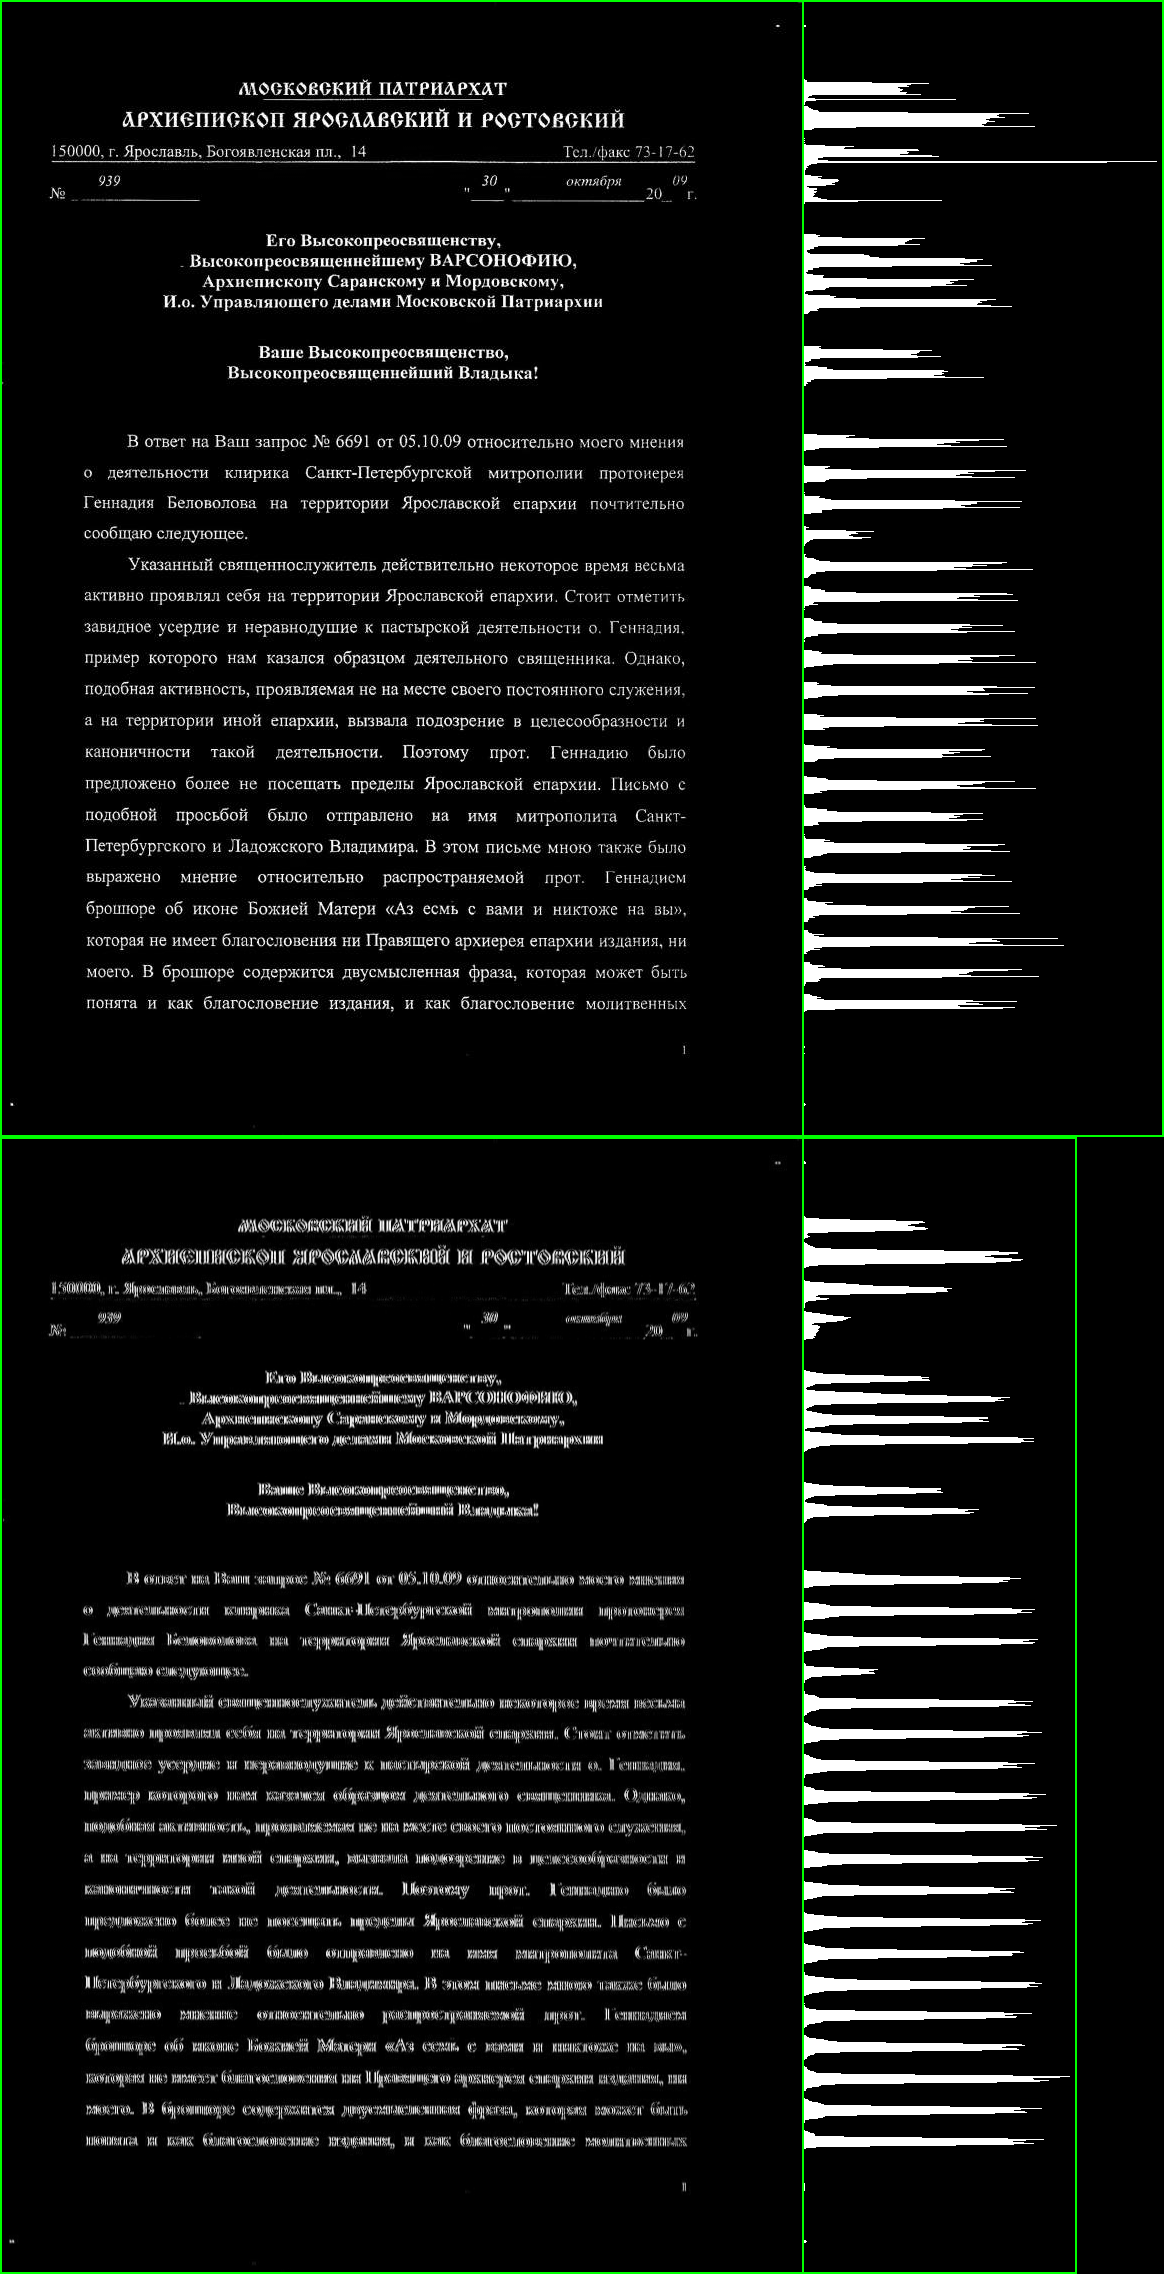
\includegraphics[scale=0.7]{output-gradient.png}

\end{document}